\chapter{Knowledge}
\label{cha:knowledgei}

\section{Prerequisites}
This section will introduce some important knowledges, including sigmoid function, Bayes Formula, Huffman code, etc.

\subsection{Sigmoid Function}
Sigmoid function is a common kind of active function, the definition is
$$ \sigma(x) = \frac{1}{1+e^{-x}}, $$
The domain is $(-\infty, \infty)$, the range is $(0,1)$. And Figure~\ref{fig:sigmoid} shows the sigmoid function.
\begin{figure}[!ht]
  \centering
	\fbox{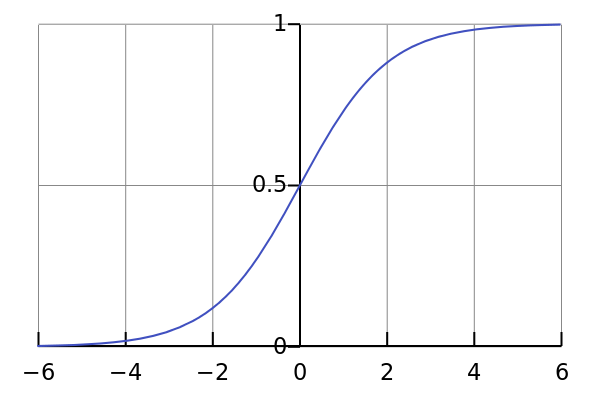
\includegraphics[width=0.5\textwidth]{sigmoid} }
	\caption{Sigmoid Function}
	\label{fig:sigmoid}
\end{figure}

Sigmoid function has the \textbf{derivative function} as following:
$$ \sigma^\prime(x) = \sigma(x)[1-\sigma(x)], $$
Thus, the \textbf{derivative functions} of $\mathrm{log}\sigma(x)$ and $\mathrm{log}(1-\sigma(x))$ are respectively
\begin{equation} 
[\mathrm{log}\sigma(x)]^\prime = 1-\sigma(x), \ [\mathrm{log}(1-\sigma(x))]^\prime = -\sigma(x), 
\end{equation}
Equation (2.1) will be used later in derivations.

\subsection{Logistic Regression}
Binary classification is a very common task, for example, if an email is spam, if a customer is a potential customer, if a online transaction fraud, etc. Let ${\{(\mathbf{x}_i,y_i)\}}^m_{i=1}$ be the sample data of a binary classification problem, where $\mathbf{x}_i \in \mathbb{R}^n$, $y_i \in \{0,1\}$, when $y_i = 1$ the corresponding sample is $\mathbf{positive}$, when $y_i = 0$ the corresponding sample is $\mathbf{negative}$.

As for some sample data $\mathbf{x} = (x_1,x_2,\cdots,x_n)^T$, the hypothesis function can be written as
$$h_\theta(\mathbf{x}) = \sigma(\theta_0+\theta_1 x_1+\theta_2 x_2+\cdots+\theta_n x_n),$$
where $\theta = (\theta_0,\theta_1,\cdots,\theta_n)^T$ is undetermined parameters. To simplify the formula, one can introduce $x_0 = 1$, and then $\mathbf{x}$ is extended to $(x_0,x_1,x_2,\cdots,x_n)^T$. Without confusing one can also record it as $\mathbf{x}$. Thus, $h_\theta$ can be simplified as 
$$h_\theta(\mathbf{x}) = \sigma(\theta^T \mathbf{x}) = \frac{1}{1+e^{-\theta^T \mathbf{x}}}.$$

Let threshold $T = 0.5$, then the discriminant formula for binary classification is
$$y(\mathbf{x})=
\begin{cases}
1,& h_\theta(\mathbf{x})\geq 0.5;\\
0,& h_\theta(\mathbf{x})\le 0.5.
\end{cases}$$

How to calculate $\theta$ ? A common method is, firstly one defines a form of the \textbf{overall loss function} as following
$$ J(\theta) = \frac{1}{m}\sum^m_{i=1}cost(\mathbf{x}_i,y_i),$$
and then one optimizes the overall loss function to obtain the optimal parameters $\theta^*$.

In practice, the loss function of a single sample $cost(\mathbf{x}_i,y_i)$ is often taken as the \textbf{log-likelihood function}
$$cost(\mathbf{x}_i,y_i)=
\begin{cases}
-\mathrm{log}(h_\theta(\mathbf{x}_i)),& y_i=1;\\
-\mathrm{log}(1-h_\theta(\mathbf{x}_i)),& y_i=0.
\end{cases}$$
Note that the above formula is a piecewise function, which can also be written in its overall expression as following
$$cost(\mathbf{x}_i,y_i) = -y_i\cdot\mathrm{log}(h_\theta(\mathbf{x}_i))-(1-y_i)\cdot\mathrm{log}(1-h_\theta(\mathbf{x}_i)).$$

\subsection{Bayes Formula}
Bayesian formula is put forward by the British mathematician Thomas Bayes, used to describe the relationship between two conditional probabilities. Let $P(A)$ and $P(B)$ respectively be the probability of event A and the probability of event B, $P(A|B)$ be the probability of the event A when event B occurs, and $P(A,B)$ be the probability of event A and B occurring simultaneously, so we have
$$P(A|B)=\frac{P(A,B)}{P(B)}, P(B|A)=\frac{P(A,B)}{P(A)}, $$
further, we can get
$$P(A|B)=P(A)\frac{P(B|A)}{P(B)},$$
the above formula is the \textbf{Bayes formula}.

\subsection{Huffman Coding}

\subsubsection{Huffman Tree}
In computer science, \textbf{tree} is a kind of nonlinear data structure, from which data elements (called \textbf{nodes} in the tree) organized in branch. The collection of several disjoint trees is called \textbf{forest}. The following concepts are some common concepts about tree.
\begin{itemize}
\item \textbf{Path} and \textbf{Path Length}\\
In a tree, a path is a road from any node to its direct or indirect child. The number of branches is called path length of the path. If the layer of the root node is $1$, the path length from the root node to nodes in the layer $L$ is $L-1$.
\item \textbf{Weight of a Node} and \textbf{Path Length with Weight of a Node}\\
Giving a node in a tree some value (non-negative), this value is called the weight of the node. The path length with weight of a node is the product of the path length from the root node to this node and the weight of this node.
\item \textbf{Path Length with Weight of a Tree}\\
The path length with weight of a tree is the sum of path length with weight of every leaf node.
\end{itemize}

A \textbf{Binary tree} is an ordered tree in which each node has at most two sub-trees. Two sub-trees are usually called \lq\lq Left Sub-Tree\rq\rq\ and \lq\lq Right Sub-Tree\rq\rq , the \lq\lq ordered\rq\rq\ means the order of left and right can not be reversed for two sub-trees.

Giving $n$ weights as weights of $n$ leaf nodes, one can build a binary tree. From all built trees, the one with the smallest path length with weight is called \textbf{Optimal Binary Tree}, which is also named \textbf{Huffman Tree}.
\subsubsection{Huffman Tree Construction}
Giving $n$ weights $\{w_1,w_2,\cdots,w_n\}$ as $n$ leaf nodes, one can build a Huffman tree as the following algorithm.\\

\noindent \ \ \ \textbf{Algorithm 2.1} (\emph{Huffman Tree} Construction)
\begin{enumerate}
\item Consider $\{w_1,w_2,\cdots,w_n\}$ as root weights of $n$ trees in a forest (each tree has only one node).
\item Select the two trees in the forest with the smallest root weight, and combine them to be a new tree. These two trees are the left and right sub-trees of the new tree, and the root weight of the new tree is the sum of root weights of its sub-trees.
\item Remove above two trees from the forest, and add the new tree into the forest.
\item Repeat Step 2 and Step 3, until there is only one tree in the forest. Such tree is the \emph{Huffman Tree}.
\end{enumerate}

The following example is about Algorithm 2.1.
\subsubsection{Huffman Coding}

%--------------------------------------------------------------------------------------------------------------------------------%

\section{Skip-gram model}


